\documentclass[12pt,a4paper]{article}
\usepackage[margin=1in]{geometry}
\usepackage[utf8]{inputenc}
\usepackage{booktabs} % for toprule, midrule and bottomrule
\usepackage{adjustbox}
\usepackage{amsmath}
\usepackage{etoolbox}
\usepackage{setspace} % for \onehalfspacing and \singlespacing macros
\usepackage[hidelinks]{hyperref}
\usepackage{array}
\usepackage{graphicx}
\usepackage{setspace}
\usepackage{caption}
\usepackage{pdflscape}
\usepackage{caption}
\usepackage{tabularx}
\usepackage{authblk}
\usepackage{float}
\usepackage{siunitx}
%\usepackage{showframe}
\usepackage{titlesec}
%\usepackage{lipsum}

% set space
\doublespacing

% section headings
\renewcommand{\thesection}{\Roman{section}.\hspace{-0.5em}}
\renewcommand\thesubsection{\Alph{subsection}.\hspace{-0.5em}}


\titleformat{\section}
{\bf\centering\large}{\thesection}{1em}{}

\titleformat{\subsection}
{\itshape\centering}{\thesubsection}{1em}{}


% booktabs
\setlength\heavyrulewidth{0.06em} % 0.01em> midrule

% images
\graphicspath{ {D:/Users/saketh/Documents/GitHub/OrderRoutingAndPFOF/exhibits/} }

% array
\newcolumntype{L}[1]{>{\raggedright\let\newline\\\arraybackslash\hspace{0pt}}m{#1}}
\newcolumntype{C}[1]{>{\centering\let\newline\\\arraybackslash\hspace{0pt}}m{#1}}
\newcolumntype{R}[1]{>{\raggedleft\let\newline\\\arraybackslash\hspace{0pt}}m{#1}}

% caption set up
\captionsetup[table]{
	font = {sc},
	labelfont = {sc}
}

% sig stars
\def\sym#1{\ifmmode^{#1}\else\(^{#1}\)\fi}

% hyperlinks
\hypersetup{
	colorlinks=false
}

% bibliography
\makeatletter
\renewenvironment{thebibliography}[1]
{\section*{References}%
	\@mkboth{\MakeUppercase\refname}{\MakeUppercase\refname}%
	\list{}%
	{\setlength{\labelwidth}{0pt}%
		\setlength{\labelsep}{0pt}%
		\setlength{\leftmargin}{\parindent}%
		\setlength{\itemindent}{-\parindent}%
		\@openbib@code
		\usecounter{enumiv}}%
	\sloppy
	\clubpenalty4000
	\@clubpenalty \clubpenalty
	\widowpenalty4000%
	\sfcode`\.\@m}
{\def\@noitemerr
	{\@latex@warning{Empty `thebibliography' environment}}%
	\endlist}
\makeatother

% etoolbox
\AtBeginEnvironment{quote}{\singlespacing\small}

\begin{document}
	
\title{\textbf{The Effect of Payment for Order Flow} \\ \vspace{-0.5em} \textbf{on Order Routing}}

\author[]{Saketh Aleti}

\affil[]{Advisor: Professor Bruce Mizrach}

\maketitle


\section{Introduction}	

One of the most significant changes in US equity markets in the last decade is the emergence of widespread competition for retail order flow\footnote{ Retail order flow refers to orders for securities that originate from retail investors as opposed to institutional investors such as banks and hedge funds}. About 20 years ago, stocks listed on an exchange such as NASDAQ were only traded on that exchange. Today, when a broker receives an order, they can redirect the order to one of hundreds of locations or internalize\footnote{ Internalization is the process by which a broker executes an order against their own inventory, so they can profit from the difference between the order's price and the market price} it. If they choose to redirect the order, it may go to an exchange, a market maker, or an electronic communications network. 
The SEC refers to these venues as \textit{market centers}; they define a market center as ``any exchange market maker, OTC market maker, alternative trading system, national securities exchange, or national securities association" as per the Securities Exchange Act of 1934.
Most venues offer brokers some rebate, usually less than a penny per share, in order to attract order flow.  The process by which market centers offer rebates for orders from broker-dealers is called \textit{payment for order flow} (POF). This practice remains controversial, since it allows brokers to effectively sell their client's orders to the highest bidder rather than sending them to the market center with the best execution. At the same time, some have argued that payment for order flow has come with benefits such as greater exchange competition (Angel, Harris, and Spatt, 2011). 


According to an industry notice from the National Association of Securities Dealers, now the self-regulatory agency FINRA,


\begin{quote}
	The traditional non-price factors affecting the cost or efficiency of executions should also continue to be considered; however, broker-dealers must not allow an order routing inducement, such as payment for order flow or the opportunity to trade with that order as principal, to interfere with its duty of best execution. (2001)
\end{quote}
The SEC has made similar statements and codified certain requirements for the processing of order flow. Between 2005 and 2007, the SEC updated the Securities Exchange Act of 1934 with Regulation National Market System (Reg NMS); this regulation introduced new rules for order protection, intermarket access, sub-penny pricing, and market data. In particular, according to the SEC's Order Protection Rule of Reg NMS, orders must be executed at the National Best Bid or Offer (NBBO) or better; the best bid is the highest price a buyer will accept and the best offer is the lowest price a seller will accept. This rule establishes price priority, so brokers cannot\footnote{ There are exceptions for this rule which are aimed at High Frequency Traders, but this is irrelevant for retail order flow.} execute their client's orders at a worse price than the NBBO. However, when multiple exchanges are trading a stock at the NBBO, the broker can choose which venue to route to. 

In such a case, brokers may decide where to route based on the rebate they receive for directing order flow. This involves responding to one of two fee structures: either payment for order flow or maker-taker fees. The latter simply involves paying a fee for removing liquidity (sell orders) and receiving a rebate for adding liquidity (buy orders). This fee/payment structure is particularly targeted towards limit orders. On the other hand, payment for order flow consists of purchasing orders independent of whether they are buy or sell; generally, this is targeted towards all order types. 
For the sake of a retail investor, it would be best if brokers routed their clients' orders to maximize their execution quality; 
for instance, they ought to optimize execution quality factors such as price improvement, execution speed, execution probability, and so on. Brokers are incentivized to do so, because offering a better service should win them more clients; also, legally, they are supposed to route orders to where they would receive the best execution. But, there exists enough leniency within the SEC's definition of a ``best execution" under Reg NMS for brokers to route according to their own objectives and offer a post hoc justification. 

My thesis aims to identify how the presence of payment for order flow affects order routing. 
So, I examine the responsiveness of different subgroups of brokers to changes in the execution quality of market centers. 
Some brokers happen to accept payment for order flow while others do not; this makes it possible to compare the order routing of \textit{paid} (payment-accepting) brokers versus \textit{unpaid} brokers, and thus the identify the effect of payment for order flow. 
I expect that all brokers route a greater percentage of orders towards market centers with better factors of execution quality such as higher price improvement or faster execution speed. In particular
In particular, I hypothesize that paid brokers are less responsive than unpaid brokers to changes in execution quality. That is, payment for order flow has a negative effect the executions of retail orders directed by paid brokers. This research expands upon previous research in market microstructure that studies the effects of rebates and fees offered firms looking to capture order flow.  



\section{Literature Review}	

\subsection{The Theoretical Foundation for Order Rebates}

Early research on the effects of payment for order flow is still relatively recent given that the practice emerged in the 1980s. At that time, order flow payments were as high as a penny per share, since major exchanges would trade in $12.5$ cent increments. As a result, the early literature, such as Chordia and Subrahmanyam (1995) and Kandel and Marx (1999), argued that payment for order flow was caused by higher tick sizes. However, as tick sizes got smaller, payments did not disappear but simply diminished in size. Now, newer papers like Parlour and Rajan (2001) and Battalio and Holden (2001) present theoretical models for the existence of payments for order flow persisting in continuous price settings. 

In particular, Battalio and Holden find that brokers can maximize profits by using their internal data on their clients to identify uninformed order flow; if a broker predicts that their client is uninformed, they internalize the order and profit from the spread. On the other hand, their model assumes that third parties, such as market centers, purchase order flow based on ``externally-verifiable" characteristics; this is a realistic assumption given that third parties do not have access to client data before they purchase an order. These factors motivate third parties to pay for order flow, since they will only have access to potentially uninformed order flow if they can compete with internalization. The former paper, Parlour and Rajan (2001), develops another theoretical model consisting of an infinite horizon game of liquidity-provision. This game consists of competing market makers, brokers, and investors; market makers supply liquidity, investors demand or supply liquidity, and brokers act as intermediaries. Their model finds that scenarios where payment for order flow is allowed results in lower consumer and social welfare than the counterfactual. Additionally, its existence results in a welfare transfer from liquidity takers to suppliers, which they define as those submitting market orders versus those sending limit orders. Both models hold the number of market centers fixed, while there also exists literature on the effects of greater competition as well. 

\subsection{The Effects of Order Rebates}

Angel, Harris, and Spatt (2011) note that Regulation NMS has resulted in significantly greater competition among market centers. However, Dennert (1993) and Duta and Madhavan (1997) find that competition between market centers can actually have mixed effects for retail investors. Firstly, Dennert (1993) models price competition where prices are quoted by competing dealers facing some unknown future demand. Then, introducing informed and uninformed traders to the model, Dennert finds that increasing the number of market makers increases their individual risk exposure. As a result, bid-ask spreads increase and liquidity traders face higher transaction costs. So, there exist cases where liquidity traders, who are generally uninformed, would be better off in monopolistic markets than competitive ones. Next, Duta and Madhavan (1997) present a model where multiple market makers compete with one another resulting in higher spreads; in some ways, this effect is similar to what would occur if the market makers colluded and fixed prices. They suggest that this outcome is due to current institutional arrangements, and investors would be better off if price priority was eliminated, internalization was discouraged, and order flow payments were eliminated. 

Other papers find similar results regarding the effect of order rebates. Cimon (2016) presents a theoretical model of limit order trading and finds that significant spreads in the fee/rebate for maker-taker venues cause brokers to reroute orders to venues with poor execution quality. This model consists of two periods where brokers decide where to route their clients marketable orders. The paper then provides a theoretical basis for two empirical results: exchanges with higher rebates will endogenously have worse fill rates and, when trading fees are sufficiently different, brokers will prioritize rebates over their clients' orders fill rates. Maglaras, Moallemi, and Zheng (2015) develop a different model where, instead of brokers acting as an intermediary, investors route their own orders and can pay fees or accept rebates for their order flow. The model finds that limit orders sent to high fee venues still face worse execution quality even when investors themselves are making the decision. Additionally, when fill rates between high and low fee venues are significantly close, routing to capture rebates is welfare improving for investors. In other cases, the rebates offered by high fee venues are not enough to offset their subpar execution quality. In short, both papers imply that maximizing rebate revenue is not equivalent to maximizing execution quality. 

Lastly, there exists literature examining the effect of maker-taker and payment for order flow models on execution quality. To begin, we have Battalio, Shkilko, and Van Ness (2016), which examines differences between venues that pay for order flow and those that use the maker-taker model in US options markets. Using trade and quote data for options from OPRA, they find that the cost of liquidity is approximately 40 basis points lower in markets that pay for order flow than those that use maker-taker. Additionally, they find that high priced options face lower spreads in maker-taker exchanges; therefore, they argue that brokers cannot fulfill their best execution obligation if they route all their orders to venues that use the payment for order flow model, which would maximize broker revenue. Analyzing US equity markets instead, Battalio, Corwin, and Jennings (2016), find empirical evidence that brokers who route to maximize rebates cannot be maximizing execution quality. Using a proprietary data set of orders, they develop a model which they then further investigate with the larger TAQ dataset. Battalio, Corwin, and Jennings find that four major retail brokers ``appear to route all non-marketable limit orders to the venue offering the largest rebate." Additionally, based on results from their proprietary data set, they find that limit order execution quality is negatively correlated with an exchange's rebate. Generalizing to the TAQ dataset, they also find that order rebates have greater impacts on low-priced stocks. In any case, these papers develop an empirical foundation for the argument that maximizing rebate revenue does not maximize execution quality. 

Based on previous literature, I expect order routing that prioritizes rebate revenue to be subpar in execution quality. As stated above, this has both a theoretical foundation and an empirical foundation. This paper aims to estimate the effect of payment for order flow on broker order routing. In the methodology section, I explain how this question can be approached by studying the effects of execution quality on the order routing. While the literature explains the theoretical effects of revenue-maximizing order routing, this research will estimate the actual effects of the presence of payment for order flow on order routing and execution quality. Thus, the results further develop the empirical literature and may offer new questions for theory. 






	
	
\section{Data Description}

	My methodology aims to quantify the effect of POF on order routing and its execution quality; in order to do so, I examine differences in order routing between brokers who do and do not accept POF. So, I use data on order routing - available through 606 disclosures - and execution quality - found in 605 disclosures.  After collecting the data, I merge both into a dataset where each observation belongs corresponds to a specific broker, market center, exchange, and time period. Because the data sets are in different time frequencies, I consolidate each to quarterly before merging. 
	
	\subsection{605 Data}
	
	

		
		\begin{table}[t]
		
		\captionsetup{}
		\caption{\small{Summary Statistics for Execution Quality Variables from 605 Data} }
		\centering
		\footnotesize
		
		\begin{tabular}{@{}L{17.85em}rrrrrrr@{}}
			\\[-4.5ex]
			\toprule
			\textbf{Execution Quality Variables} &     Mean &     Min &      25\% &      50\% &      75\% &      Max \\
			\midrule
			\multicolumn{7}{@{}l}{\textit{NASDAQ Listed Stocks}} \\ \\[-2.5ex] 
			\hline \\[-1.8ex] 
			Average Price Improvement & 0.01686 & 0.00532 & 0.01232 & 0.01619 & 0.02439 & 0.02792 \\
			Percent Price Improved    & 0.90061 & 0.84150 & 0.87148 & 0.89940 & 0.93454 & 0.94903 \\
			Expected Price Improvement & 0.01533 & 0.00483 & 0.01065 & 0.01471 & 0.02283 & 0.02485 \\
			Execution Time for Price-Improved   & 0.02909 & 0.00112 & 0.00445 & 0.00643 & 0.02577 & 0.14270 \\
			Execution Time for All Shares     & 0.03920 & 0.00192 & 0.00593 & 0.01104 & 0.03381 & 0.19163 \\
			\hline \\[-1.8ex] 
			\multicolumn{7}{@{}l}{\textit{NYSE Listed Stocks}} \\ \\[-2.5ex] 
			\hline \\[-1.8ex] 
			Average Price Improvement & 0.00672 & 0.00198 & 0.00420 & 0.00648 & 0.00893 &  0.01571 \\
			Percent Price Improved    & 0.86290 & 0.03728 & 0.85863 & 0.91970 & 0.94968 &  0.98118 \\
			Expected Price Improvement & 0.00589 & 0.00038 & 0.00349 & 0.00560 & 0.00822 &  0.01337 \\
			Execution Time for Price-Improved   & 0.17096 & 0.00000 & 0.00549 & 0.02482 & 0.19239 &  5.88234 \\
			Execution Time for All Shares     & 0.25787 & 0.00119 & 0.01197 & 0.04829 & 0.21703 & 10.47223 \\
			\hline \\[-1.8ex] 
			\multicolumn{7}{@{}l}{\textit{Other Exchange Listed Stocks}} \\ \\[-2.5ex] 
			\hline \\[-1.8ex] 
			Average Price Improvement & 0.00763 & 0.00211 & 0.00468 & 0.00707 & 0.01043 &  0.02097 \\
			Percent Price Improved    & 0.85806 & 0.10056 & 0.86543 & 0.91431 & 0.94413 &  0.97043 \\
			Expected Price Improvement & 0.00658 & 0.00047 & 0.00375 & 0.00586 & 0.00962 &  0.01643 \\
			Execution Time for Price-Improved   & 0.26946 & 0.00000 & 0.01457 & 0.04944 & 0.21461 & 11.01870 \\
			Execution Time for All Shares     & 0.42925 & 0.00000 & 0.02612 & 0.07975 & 0.29440 & 24.48855 \\
			\hline \\[-1.8ex]  
			\multicolumn{7}{@{}l}{\textit{All Stocks}} \\ \\[-2.5ex] 
			\hline \\[-1.8ex] 
			Average Price Improvement & 0.00874 & 0.00198 & 0.00506 & 0.00735 & 0.01102 &  0.02919 \\
			Percent Price Improved    & 0.85594 & 0.03728 & 0.85517 & 0.91201 & 0.94231 &  0.98118 \\
			Expected Price Improvement & 0.00757 & 0.00038 & 0.00415 & 0.00632 & 0.00993 &  0.02759 \\
			Execution Time for Price-Improved   & 0.21421 & 0.00000 & 0.00871 & 0.03785 & 0.19885 & 11.01870 \\
			Execution Time for All Shares     & 0.34278 & 0.00000 & 0.01935 & 0.06566 & 0.25043 & 24.48855 \\
			\hline \\[-1.8ex] 
			\multicolumn{8}{@{}p{\textwidth}@{}}{\textit{Note: } The table reflects statistics for market orders with a size code of 21 (executions between 100-499 shares). Price improvement is given in \$/share and execution time is given in seconds. }  \\ 
		\end{tabular}
		
		
	\end{table}
		
				Firstly, I obtain the 605 disclosures from each market center's website. The SEC requires market centers to disclose information every month regarding the quality of executions for each stock; these disclosures are referred to as 605 filings in accordance with Rule 605 of Reg NMS. The 605 data contains the volume of each stock for each order type that passes through the market center. Additionally, it breaks this volume down into orders that received price improvement,\footnote{  When an order receives price improvement, it means that the buyer/seller received a better price than what they were willing to pay or what the market offered (the NBBO); for instance, if the NBBO for \$AAPL is at $100/101$, market centers that execute trades between these prices provide price improvement.} orders that were at-the-quote, and orders that were outside-the-quote.\footnote{  ATQ refers to orders at the NBBO, while OTQ refers to orders outside the NBBO.} This data is further broken down into the number of price improved shares for each stock, the average amount of price improvement, and the average time a price improved order took to execute. Similarly, market centers report the average time and shares of at-the-quote and outside-the-quote orders as well. This data is necessary in constructing my independent variables which are measures of execution quality. Also, since 605 disclosures are reported on a monthly and per stock basis, I convert them to a quarterly and per exchange basis to match the 606 data. Lastly, I subset the data for orders with the size code 21, which refers to those between 100-499 shares; this is the smallest order size category available and likely best represents executions for the orders of retail investors. Table 1 provides summary statistics from the 605 data for the execution quality variables I use in my regressions.
		
	\subsection{606 Data}
	
		Similarly, the SEC requires broker-dealers to disclose where they route their orders and the average payment that they receive; these disclosures are referred to as 606 filings. The 606 data shows the percent of orders, by order type, that was routed to each market center. For example, Table 2 was produced from TD Ameritrade's 606 disclosure for NASDAQ stocks during the third quarter of 2017. 
		


		\begin{table}[t]
			
			\caption{\small{Example of 606 Disclosure (TD Ameritrade, NASDAQ, 2017Q3)}}
			\centering
			\footnotesize

				\begin{tabular}{@{} l   C{2.5cm}  C{2.5cm}  C{2.5cm}  C{2.5cm} @{}}
					\\[-4.5ex]
					\toprule
					& \multicolumn{4}{c}{{\textbf{Order Type}}} \\ 
					\cline{2-5} \\ [-1.8ex]
					\textbf{Routing Venue} & Total & Market  & Limit &  Other  \\ 
					\hline \\[-1.8ex] 
					TD Ameritrade Clearing & 77\%  & 85\% &  74\%  & 72\%   \\ 
					Citadel Execution Services &  13\% &  9\%  & 14\%  & 17\%   \\
					Virtu Americas, LLC  & 6\% &  4\%  & 6\%  & 8\%   \\ 
					Citi Global Markets  & 3\%  & 0\%  & 5\% &  0\%   \\ 
					Two Sigma Securities, LLC  & 1\%  & 2\%  & 1\%  & 3\%   \\ 
					[0.2ex] \hline
				\end{tabular}
				\\[-1.8ex]
		\end{table}
		
		Also, note that TD Ameritrade redirects a majority of its orders to its own clearing corporation, which itself produces a 606 disclosure documenting its order flow; this is a fairly common practice among the larger brokers. In order to account for order flow from a broker to its subsidiary clearing corp, I take the order flow payments made to the clearing corporation (found in their separate 606 filing), weight them by the share of orders sent to the clearing corp, and add them back to the order flow payments to the broker. This ensures that order flow sent to subsidiaries is accounted for in the final dataset. For instance, if TD Ameritrade Clearing sends 50\% of its orders to Citadel, then the total percent of orders routed to Citadel is 51.5\% (77\% * 50\% + 13\%).  
		
		Along with this information, the disclosure states the average payment received by TD Ameritrade from each routing venue; this is the payment for order flow. However, this variable is a deterministic function of the order routing already present in the data. That is, market centers pay different amounts for different types of orders. The average payment reported by brokers is the total payment received divided by the number of shares routed to a certain market center. So, if a market center offers higher rebates for market orders than limit orders and a broker routes more market orders their way in some future time period, then the average payments reported would increase even though the actual rebates offered may not have changed. This makes it impossible to draw any information from the average payments statistic without an endogeneity problem. Additionally, more specific data regarding payment for order flow is unavailable, so there is no way of extracting any information from average payments alone. Instead, I simply keep track of which brokers offer order rebates with a dummy variable; brokers, legally, must disclose if they are receiving payment for order flow, so this data is available. I use this later on for a subgroup analysis. 
		
		It is also important to note that order routing requires particular infrastructure to process which limits the universe of market centers that brokers can route; this requires adjusting the raw 606 data. Returning to the TD Ameritrade example, they route to Citadel, Virtu, Citi, and Two Sigma, although many other potential market centers exist. One approach to filling in the discluded entries would be to populate the 606 data with 0\% entries for all market centers available from the 605 data. However, this would ignore the issue of infrastructure. A broker may set up a connection to a new market center if they believed that they would receive marginally better execution quality by doing so. And, setting up a connection is a fixed cost and the connection likely persists for some time even after brokers cease to route to a market center. So, I adjust the 606 data to include missing zeros by only adding entries for market centers that a broker has routed to in the past two quarters. This ensures that regressions on this data avoid selection bias while taking infrastructure into consideration. 
		
		Lastly, some brokers did not accept payment for order flow but were still included under the subgroup \textit{POF brokers}. This was done when brokers routed to clearing corporations that received payment for order flow. For instance, Hollencrest Securities receives no POF, but contracts Charles Schwab to route its orders; the latter do accept POF. Hence, Hollencrest's order routing is still implicitly under the influence of rebates although it receives none. So, I use the term \textit{POF} or \textit{paid} in the sense that these types of brokers' order routing is affected by POF whether or not they actually receive any direct financial compensation. On the other hand, those not under the influence of payment for order flow are referred to as \textit{Non-POF} or \textit{unpaid} brokers. 
		
		In total, the 606 data provides order routing data, or ``market share" within brokers, for each market center specified by exchange and order type on a monthly basis. 


	

\section{Methodology}

	My analysis identifies the effect of POF on order routing by comparing brokers who accept/reject POF in terms of their responsiveness to changes in execution quality. I do so by regressing market share on execution quality; their responsiveness is measured by the magnitude of their execution quality coefficients in the regressions. The difference between the coefficients of brokers who do and do not accept POF indicates the extent to which order routing differs under the presence of POF. I estimate my model using a Tobit regression and a semiparametric least squares approach. 

	\subsection{Model Formulation}

	Suppose that brokers route orders based on a the market center's execution quality and its payment for order flow; realistically, these are the only possible variables a profit-maximizing firm would take into account besides for some sort of personal relationship with a market center. That sort of effect would be fixed over time, so it can be modeled with a constant term. So, in total, we have fixed effects represented by $\alpha$, a vector of execution quality factors represented by $X$, and the level of payment for order flow denoted by $Z$; these variables determine $Y$ which denotes market share - the percent of orders routed by a broker to a particular market center. 
	\begin{equation}
	Y_{i, j, k, t} = \alpha_{i,j,k} +  X_{j, k, t} \cdot \beta +   Z_{j,  t} \cdot \gamma + \varepsilon
	\end{equation}	
	
	The subscript $i$ denotes the broker, $j$ denotes the market center, and $k$ denotes the exchange. Lastly, we have $\epsilon$ representing the error term.
	

	In this model, the term $Z$, payment for order flow, is unknown because there is no data available to construct it. This could cause omitted variable bias if $\gamma \neq 0$ and $cov(X, Z) \neq 0$. However, although the former I hypothesize to be true, I believe that the latter is not. This is because $Z_{j,  t}$ states the level of rebate offered for order flow at some point in time $t$. For it to have a causal relationship with $X_{j, k,  t}$, we would need market centers either reacting to execution quality shifts by changing rebates and/or responding to rebate revenue with changes in execution quality. The latter is impossible, because market centers cannot simply choose how well trades are executed on their markets. Better trade-matching algorithms may lead to better executions, but market centers cannot `undo' investments into improving their execution quality nor are these straightforward investments with consistent, short-term returns in execution quality. So, if rebate revenue increased, a market center cannot cut costs by reducing execution quality; and, if it decreased, it is improbable that a market center could simply better its execution quality in the same period. Additionally, improvements in execution quality tend to be a result of technological process (such as faster computers); its non-trivial for a market center to improve execution quality by any premeditated amount. On the other hand, it is also unlikely that market centers can respond to execution quality changes by changing their rebates. This is because market centers cannot change their rebates very often; there's a significant amount of paperwork involved and it can take several quarters for changes in the rebate structure to actually go through. So, market centers cannot react well to changes in execution quality by changing the prices they offer for rebate flow. Moreover, it is very difficult to predict when execution quality will fall, and, even if predicted, it may be a result of systemic problems in the market rather than being particular issue with the market center itself. In short, $cov(Z, X)$ is likely $0$. Moreover, $\gamma$ will trivially equal $0$ for unpaid brokers, so regressions on their subgroup will remain consistent even without this assumption. 
	
	Second, with respect to the factors of execution quality, $X$, I construct this variable using data on price improvement and execution time through the 605 disclosures. Considering price improvement, I have data on the number of price-improved shares, the average amount of price improvement, and the average time that price-improved shares took to execute. I use the latter two in my regressions, and I use the former to construct the percent of shares that were price-improved. Additionally, I include an interaction term between percent of price-improved shares and average price improvement; their product is the expected amount of price improvement. Additionally, since the data shows the average time that all types of executions took, I construct a variable for the average time that a share takes to execute at a market center. Also, I consider average effective spreads, the average difference between the NBBO spread (ask - bid) and the trade price, in my regression; tighter spreads generally indicate better executions. In total, I run several regressions using some combination of terms for the level of price improvement, a term for average time taken, and a term for spreads; I use the variables with the best explanatory power to construct the $X$ variable. 
	
	\begin{equation}
	Y_{i, j, k,  t} \,=\, \alpha_{i,j} \,+\,  X_{j, k, t} \cdot \beta \,+\,  (D_i \cdot X_{j, k, t}) \cdot \gamma\, +  u
	\end{equation}	
	\begin{equation}
	Y_{i, j, k, t} = \alpha_{i,j} +  X_{j, k, t} \cdot \beta +  v
	\end{equation}	

	Lastly, since $Y$ is defined as market share, this model is censored at 0 and 1. In the data, there are no cases where a broker routes 100\% of its orders to any market center, so only censoring at 0\% practically applies. In this case, a Tobit model would be appropriate. However, some argue that the assumption of normality is more problematic than the inconsistency caused by running OLS on censored data. So, I run OLS, Tobit, and a semiparametric model on the data, and compare the results. With respect to the OLS regression, the unobservable fixed effects may be correlated with $X$ and the large quantity of constant terms may create inconsistency. So, I consider both random effects and fixed effects and choose the appropriate model using a Hausman test. In the parametric models, I use functional forms resembling equation (2) where I regress on $X$ and $X \cdot D_i$ where $D_i$ is an indicator variable for whether a firm accepts payment for order flow. The significance of the coefficients corresponding to $X \cdot D_i$ then determines whether the coefficients for paid brokers are significantly different than unpaid brokers. If these coefficients, assuming they are significant, are negative for price improvement terms and positive for execution speed term, then the results would favor my hypothesis that Non-POF brokers route better than POF brokers; this in turn would imply that POF has a deleterious impact on order routing.And, lastly, with respect to the semiparametric least squares model (Ichimura, 1993), I regress using equation (3) using a Gaussian kernel to find $\theta = \beta / \beta_1$. Since this regression returns only the ratios between coefficients, I treat coefficient $\beta_1$, either percent price-improved or expected price improvement, as a given variable in their respective models. Then, I find the standard errors of the other variables. I perform the SLS regression on POF and Non-POF brokers separately and then compare the significance of the coefficients in each and the differences between the two in marginal effects. Significant differences in these would imply that the two types of brokers behave differently; the signs of these differences then indicate whether POF brokers perform better or worse than Non-POF brokers. 
	
	


	
\section{Results}

	 I present estimated effects of POF on execution quality in Table 3: the Tobit regression results. This effect is measured through the interaction terms with $D_i$, the POF indicator variable; I find significant differences between POF and Non-POF Brokers in terms of responsiveness to all measures of execution quality except average price improvement.\footnote{I also regressed subsets of the data by exchange. Payment for order flow seems to have slightly worse effects on the order routing of NASDAQ-listed stocks compared to those listed on the NYSE or other exchanges. This result does not appear to be significant for all fits or have any theoretical foundation.}  I get similar results from running OLS directly on the data; these regressions are reported in Table A1 in the appendix. Furthermore, in Table 4, I provide the results of SLS along with plots of marginal effects. The semiparametric approach returns similar results but with much smaller magnitudes; Non-POF brokers perform better with respect to price improvement but both types of brokers perform about equally with respect to execution speeds. The marginal effect plots show Non-POF brokers responding more strongly to changes in execution quality at worse market centers; the results are weaker for average and better market centers . 



\subsection{Effects on Execution Quality - Parametric Regressions}

\begin{table}[t] 
	\caption{Tobit Regression Results} 
	\label{} 
	\footnotesize
	\begin{tabular}{@{\extracolsep{0.6em}}lcccc} 
		\\[-4ex]\hline  
		\hline \\[-1.8ex]  
		& \multicolumn{4}{c}{\textit{Dependent variable:}} \\  
		\cline{2-5}  
		\\[-1.8ex] & (1) & (2) & (3) & (4)\\  
		\hline \\[-1.8ex]  
				Percent of Shares Price Improved   &     -0.0536         &                     &     -0.0461         &                     \\
		&     (0.129)         &                     &     (0.131)         &                     \\
		[0.5em]
		Percent of Shares Price Improved  $\times$ D$_i$  &  -0.497\sym{**} &                     &      -0.503\sym{**} &                     \\
		&     (0.191)         &                     &     (0.192)         &                     \\
		[0.5em]
		Avg Price Improvement&       14.25\sym{***}&                     &       14.18\sym{***}&                     \\
		&     (2.895)         &                     &     (2.875)         &                     \\
		[0.5em]
		Avg Price Improvement$\times$ D$_i$&      -6.677         &                     &      -7.200         &                     \\
		&     (4.279)         &                     &     (4.256)         &                     \\
		[0.5em]
		Expected Price Improvement&                     &       14.75\sym{***}&                     &       14.62\sym{***}\\
		&                     &     (3.206)         &                     &     (3.190)         \\
		[0.5em]
		Expected Price Improvement$\times$ D$_i$&                     &      -13.55\sym{**} &                     &      -13.98\sym{**} \\
		&                     &     (4.600)         &                     &     (4.578)         \\
		[0.5em]
		Avg Execution Time for Price-Improved  &      -0.117\sym{**} &      -0.116\sym{**} &                     &                     \\
		&    (0.0400)         &    (0.0402)         &                     &                     \\
		[0.5em]
		Avg Execution Time for Price-Improved$\times$ D$_i$&      0.0982\sym{*}  &       0.102\sym{*}  &                     &                     \\
		&    (0.0411)         &    (0.0413)         &                     &                     \\
		[0.5em]
		Avg Execution Time for All Shares    &                     &                     &     -0.0586\sym{**} &     -0.0581\sym{**} \\
		&                     &                     &    (0.0195)         &    (0.0198)         \\
		[0.5em]
		Avg Execution Time for All Shares $\times$ D$_i$&                     &                     &      0.0514\sym{*}  &      0.0531\sym{**} \\
		&                     &                     &    (0.0202)         &    (0.0205)         \\
		[0.5em]
		Constant      &     -0.0744\sym{***}&     -0.0757\sym{***}&     -0.0744\sym{***}&     -0.0756\sym{***}\\
		&   (0.00788)         &   (0.00782)         &   (0.00789)         &   (0.00783)         \\
		\hline \\[-1.8ex]  
		Observations & 2,982 & 2,982 & 2,982 & 2,982 \\  
		Log Likelihood & $-$955.832 & $-$984.152 & $-$959.019 & $-$986.638 \\  
		Wald Test & 96.801$^{***}$ & 38.828$^{***}$ & 91.954$^{***}$ & 35.462$^{***}$ \\  
		\hline \\[-1.8ex]  
		\multicolumn{5}{@{}p{45em}@{}}{\textit{Note: } $D_i$ denotes an indicator variable for a broker accepting POF. Robust standard errors are reported in parentheses. *p$\textless$0.05, **p$\textless$0.01, ***p$\textless$0.001}  \\ 
	\end{tabular} 
\end{table} 




Execution quality regressors multiplied by the POF indicator variable, $D_i$, produce coefficients that quantify the difference in responsiveness between POF and Non-POF brokers to their respective execution quality measure. For instance, in Table 3, the interaction term for expected price improvement in fit 4 is $-13.55$ ($|t| = 2.95$). This implies that brokers who receive payment for order flow respond significantly worse, compared to unpaid brokers, to changes in market centers' expected price improvement; thus, the presence payment for order flow likely reduces the price improvement retail investors receive compared to a counterfactual without its existence. This particular result is supported by fit 2 (Table 3) as well. And, the same findings reappear in the OLS regressions (Table A1) where the coefficient are slightly slower in magnitude but about equally significant. In the particular case mentioned earlier, a coefficient of $-13.55$ can imply a significant loss of welfare. For instance, suppose that a market center improved its expected price improvement by $\$0.01$, a moderate change. A broker accepting POF would shift their order routing to particular market center by $13.55\%$ less than a non-POF broker. If both brokers routed $100$ million shares in volume per week,\footnote{ For reference, TD Ameritrade routes more than 500,000 trades per day (Horowitz, 2014). Assuming each trade's volume was $50$ shares, this adds up to a weekly volume of $\$175$ million. This weekly volume is about as much as the daily volume for a large-cap stock.}  retail investors using the POF-broker would miss out on approximately $\$7$ million in expected price improvement per year.




On the other hand, the coefficients on the percent of orders that received price improvement were all negative and insignificant; this may be due to the lack of variation in this variable among market centers. That is, the average market center offers price improvement on $91.4\%$ of its orders, while the standard deviation of this variable between market centers is $3.5\%$. At the same time, the interaction term for average price improvement remains significant; in Table 3, there was a strong difference $(p < 0.01)$  between POF and Non-POF brokers. So, although brokers in general may pay little attention to this measure of execution quality, unpaid brokers still prioritize it more than those who receive POF. Additionally, by repeating the same exercise as with expected price improvement, we can see the $-0.497$ coefficient (Table 3: fit 1) implies major welfare losses as well. In this case, suppose we have the median market center, which offers an average price improvement of $\$0.00874$ per share. A moderate increase in the percent of shares price-improved, say by $3\%$, would translate to retail investors missing out on $\$1.3$ million per year in potential price improvement due to the presence of POF. Furthermore, this only considers losses for retail investors using that broker; generalizing to the set of all POF brokers would result in much larger potential losses. Lastly, it should be noted that there are also welfare losses implied by the significant, positive coefficients on the interaction terms for execution speed. These are probably much smaller losses and are more difficult to quantify in terms of a dollar value, since most retail investors are probably largely indifferent to whether their orders get executed within 100ms or 1s.  

In short, it seems that measures of the amount of price improvement and execution speed were relevant to all brokers, which the theoretical literature justifies.\footnote{ Some of the literature, Duta and Madhavan (1997) and Dennert (1993),  also provides a theoretical basis for including effective spreads in the analysis. So, the regressions in Table 3 and Table 4 were also performed with average effective spreads included, but these were dropped due to strong collinearity with the price improvement regressors.} Additionally, all the signs on the interaction terms were as hypothesized; only the sign on percent price-improved was unexpectedly negative. Otherwise, signs on measures of price improvement were positive, while signs were negative for execution times; and, as hypothesized, these signs were the reversed on the interaction terms, suggesting that brokers accepting POF perform worse.


\begin{table}[t] 
	\captionsetup{font=normal}
	\caption{SLS Regression Results} 
	\label{} 
	\centering
	\footnotesize
	\begin{tabular}{@{\extracolsep{0.9em}}lcccc} 
		\\[-1.8ex]\hline  
		\hline \\[-1.8ex]  
		& \multicolumn{4}{c}{\textit{Dependent variable:}} \\  
		\cline{2-5}  
		\\[-1.8ex] & (1) & (2) & (3) & (4)\\  
		\hline \\[-1.8ex] 
		\multicolumn{5}{@{}l}{\textit{Panel A: POF Brokers}} \\ \\[-2.5ex] 
		\hline \\[-1.8ex]  
		Percent of Shares Price Improved & 1 & & 1 &\\\\
		Avg Price Improvement&       1.020\sym{**} &                     &       1.061\sym{**} &                     \\
		&     (0.393)         &                     &     (0.375)         &                     \\
		[0.5em]
		Expected Price Improvement &  & 1 &  & 1\\\\
		[0.5em]
		Avg Execution Time for Price-Improved  &    0.000771         &    -0.00995\sym{***}&                     &                     \\
		&   (0.00170)         &   (0.00187)         &                     &                     \\
		[0.5em]
		Avg Execution Time for All Shares    &                     &                     &    0.000962         &    -0.00114\sym{***}\\
		&                     &                     &   (0.00167)         &  (0.000153)         \\
		\\[-1.8ex]  
		Observations & 1,494 & 1,494 & 1,494 & 1,494 \\  
		RMSE & 0.30458 & 0.30916 & 0.30466 & 0.30937 \\
		\hline \\[-1.8ex] 
		\multicolumn{5}{@{}l}{\textit{Panel B: Non-POF Brokers}} \\ \\[-2.5ex] 
		\hline \\[-1.8ex] 
		Percent of Shares Price Improved & 1 & & 1 &\\\\
		[0.5em]
		Avg Price Improvement&      -0.249         &                     &       0.711         &                     \\
		&     (0.365)         &                     &     (0.524)         &                     \\
		[0.5em]
		Expected Price Improvement &  & 1 &  & 1\\\\
		[0.5em]
		Avg Execution Time for Price-Improved  &      -0.143\sym{***}&     -0.0462\sym{***}&                     &                     \\
		&   (0.00447)         &   (0.00479)         &                     &                     \\
		[0.5em]
		Avg Execution Time for All Shares    &                     &                     &    -0.00674\sym{***}&     -0.0307\sym{***}\\
		&                     &                     &  (0.000693)         &   (0.00537)         \\
		\\[-1.8ex]  
		Observations & 1,488 & 1,488 & 1,488 & 1,488 \\  
		RMSE & 0.24503 & 0.24399 & 0.24503 & 0.24264 \\
		\hline \\[-1.8ex] 
		\multicolumn{5}{@{}p{45em}@{}}{\textit{Note: } SLS was performed using a Gaussian kernel. The data was trimmed at the 1$^{\rm st}$ and 99$^{\rm th}$ percentile, and the bandwidth and index parameters were chosen to minimize the objective function as described in Hardle, Hall, \& Ichimura, 1993.  *p$\textless$0.05, **p$\textless$0.01, ***p$\textless$0.001}  \\  
	\end{tabular} 
\end{table} 

\subsection{Effects on Execution Quality - Semiparametric Approach}



For the semiparametric approach, I regressed each subgroup independently; the results are shown in Table 5. For POF brokers, the coefficients for average execution time were highly significant but only for fits 2 and 4. Yet, in fits 1 and 3, the same  coefficients were not significant and actually positive. In the same fits, average price improvement was strongly significant; this suggests that it may be the presence of percent of shares price improved which captures much of the same variance as execution speeds. In short, brokers who accept payment for order flow are likely responsive to changes in the amount of price improvement offered, but the results are inconclusive with respect to execution speed. On the other hand, brokers who do not accept POF were highly responsive to changes in execution speeds but not necessarily to those in price improvement (Table 5: Panel B). All coefficients on regressors for execution speed were significant and negative, but those for average price improvement were not. These results suggest that POF brokers may prioritize price improvement while Non-POF brokers be more responsive to execution speed. However, since the SLS coefficients are ratios, they are not representative of the extent to which each subgroup prioritizes a particular execution quality measure.

\begin{table}[!t]
	%\caption*{} 
	\footnotesize
	\begin{tabular}{@{\extracolsep{0em}}rr}
		\multicolumn{2}{@{}c@{}}{\includegraphics[scale=0.4]{/marginaleffects/primp_pct.png} }\\
		\includegraphics[scale=0.4]{/marginaleffects/primp_avgamt.png} & 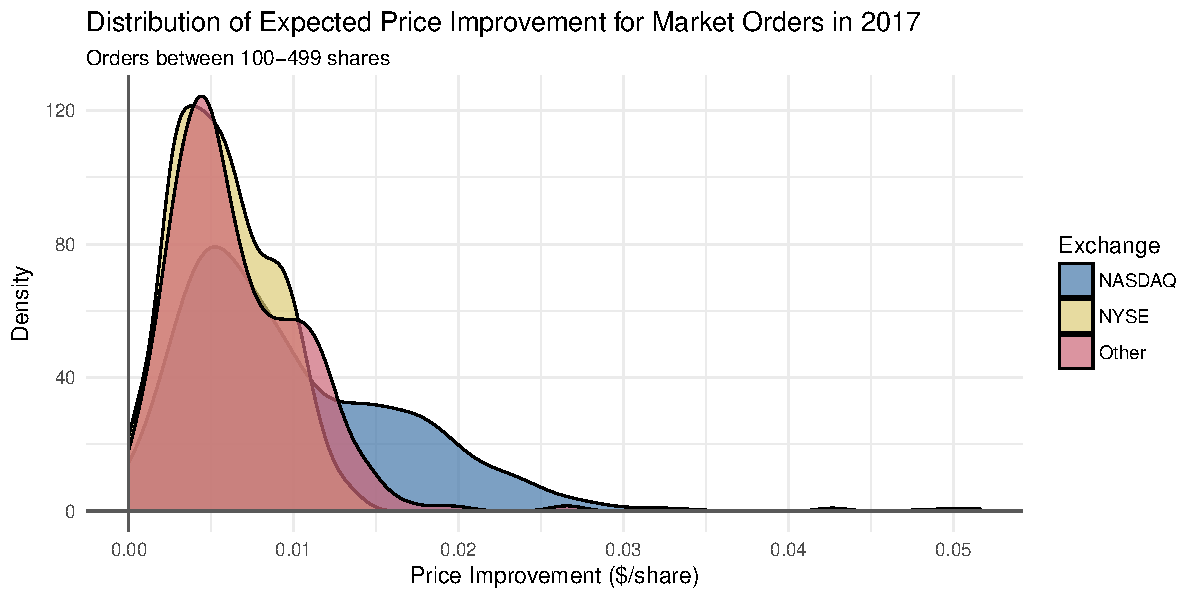
\includegraphics[scale=0.4]{/marginaleffects/primp_expamt.png} \\
		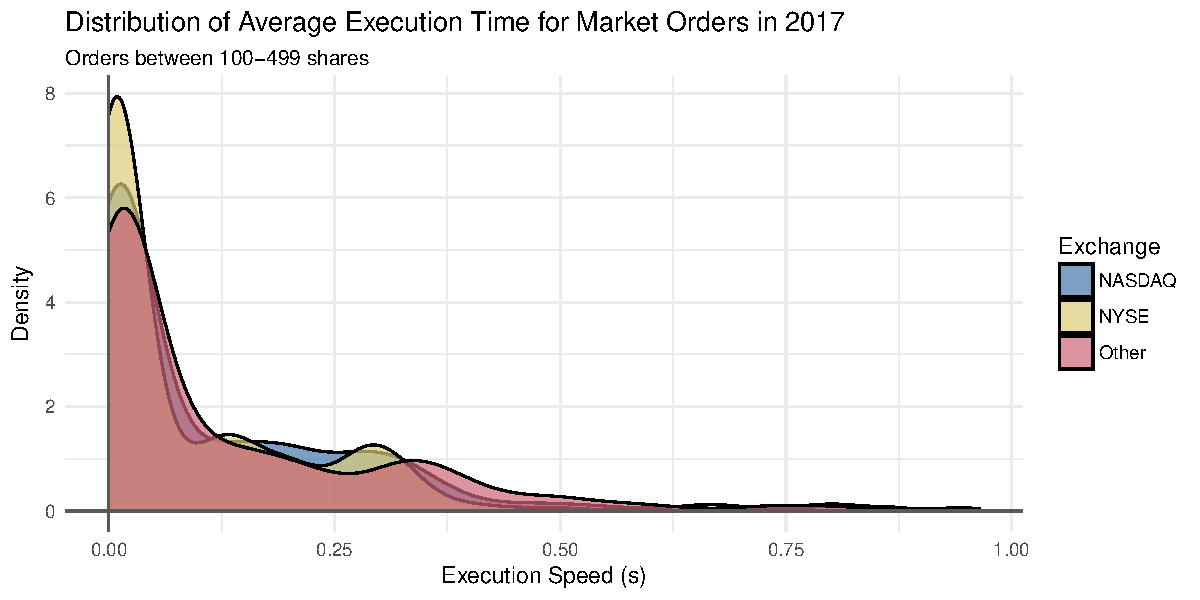
\includegraphics[scale=0.4]{/marginaleffects/primp_avgt.png} & \includegraphics[scale=0.4]{/marginaleffects/all_avgt.png} \\

		\multicolumn{2}{@{}p{6.24in}@{}}{\textit{Note: } Marginal effects were obtained using a Gaussian kernel; the bandwidth used was the same as that which minimized the objective for the SLS regressions. The solid lines represent the difference marginal effects at each percentile, while the dashed lines represent the average difference in marginal effect. For the former, execution quality percentiles were taken from the market centers receiving order flow in the data. Average marginal effects were computed by averaging the marginal effects over the execution quality data corresponding to a particular subgroup. The difference in marginal effects was taken between Non-POF and POF brokers; a positive effect then suggests a relatively higher value for Non-POF brokers.}     \\  
	\end{tabular}
\end{table}

Instead, the difference in order routing between the two can be seen through the marginal effect plots. Each figure graphs the difference in marginal effects over a range of execution quality percentiles. In the plot for average price improvement, we can see that, for both fits, Non-POF brokers outperform paid brokers at low percentiles, but this difference tapers off; the average market effect, as denoted by the dashed line, shows that Non-POF brokers are only slightly more responsive than POF brokers to average price improvement. In short, Non-POF brokers react more strongly when relatively inferior market centers start performing better but not by much. With respect to the percent of shares price-improved, we see a similar trend.  Non-POF brokers are relatively more responsive around the lower percentiles, and this difference in responsiveness decays as execution quality increases. Note that the average marginal effect is about the same as that for average price improvement; this suggests the welfare losses from POF-affected order routing towards either execution quality measure are about the same. The strongest case for a difference between POF and Non-POF brokers are found in the plot for expected price improvement. The results from fit 1 are about the same magnitude as the other price improvement measures, but the fit 3 results show a strong difference between the two broker subgroups. Lastly, the plots for execution speed show weak, positive effects in favor of POF brokers. Although this implies that POF brokers may perform better, the size of these effects is very small. That is, a 100 ms improvement in execution speeds would only be met with an average difference in market share between brokers of $0.23\%$. This is a minute effect in order routing, compared to the fact that a 100 ms change in execution speed would be a major improvement. In short, this suggests that both types of brokers are about equally responsive to changes in execution speeds.

Overall, the semiparametric results suggest a much smaller difference than what the Tobit and OLS models implied between POF and Non-POF brokers. The largest difference, the average marginal effect in fit 3 for expected price improvement ($\approx$ 4.14), implies a moderate welfare loss; the same approach from the parametric section would imply a loss, from missed price improvement, for retail investors using POF brokers of $\$2$ million per year. Similarly, for differences in order routing towards the percent of shares price-improved, the welfare losses calculated by the same approach would amount to $\$260,000$ per year. So, the semiparametric approach still finds welfare losses from payment for order flow albeit much smaller amounts. 







\section{Conclusion}



Brokers must choose to route orders either to maximize execution quality or maximize
some other objective; legally, by the SEC’s Regulation NMS, there should be no factor
besides execution quality in their order routing decisions. However, although this is in
violation of the law, brokers may route to to maximize rebates and then claim that
they maximized execution quality after the fact. Moreover, it is incredibly difficult to
prove that order flow was not routed to maximize execution quality after it is sent. The
particular state of the market at the time an order is sent affects the location where it
would receive the best execution. When brokers receive rebates, one might suspect that
their order routing suffers even though, as brokers like to argue, it is theoretically possible for a broker to accept
rebates while still prioritizing execution quality.

However, based on the results, there does seem to be a significant difference between
the order routing objectives of POF brokers and Non-POF brokers. 
The results focused on price improvement and execution speed, since these two components are likely the most important factors of execution quality, and, paid brokers, such as TD Ameritrade, even advertise these factors to clients. 
Since the coefficients of these factors differed between the two types of brokers, payment for order flow is likely causing an agency problem with rebate-accepting brokers. Rather than providing the best service for their clients, they seem to be maximizing their profit which was hypothesized. 
The particular results varied in magnitude and significance between the parametric and semiparametric approach. The parametric approach found large, significant differences between the two types of brokers in terms of routing towards measures of price improvement and execution speed. The semiparametric approach found smaller, significant differences with respect to price improvement but only minor differences for execution speeds. Overall, it seems that the welfare implications for this behavior are fairly large for price improvement but remain inconclusive for execution speeds. 

In response, brokers may make the argument that payment for order flow helps reduce
commissions. This a valid point, since commissions tend to be significantly larger than
the amount of price improvement that an investor may receive on their order. However, at
the same time, it is likely that the reduction is significantly less than the loss of execution
quality. Most retail investors are unaware of how stocks are actually executed and what
types of price improvement they should expect. As a result, we can expect the elasticity
of retail demand for a market center to be fairly low with respect to execution quality.
On the other hand, commissions are straightforward and well known. So, the elasticity
of consumer demand with respect to commissions is likely much higher. Thus, brokers
are unlikely to pass on $100\%$ of their revenue from rebates back to retail investors; the profit-maximizing approach would likely be to redirect some of the rebates to lower per-trade commissions in order to increase net profit from rebates from cheaper trades. In short,
the results from these regressions can still be used to argue that retail investors receive a
net loss in welfare from routing to POF brokers.


All in all, this study provides evidence in favor of the hypothesis that payment for order flow reduces retail investor welfare by causing brokers to miss potential price improvement. The inconclusive results with respect to execution speeds leave room for further study. One way to address this question would be to use data from the upcoming SEC Transaction Fee Pilot;
\footnote{ The pilot program would implement temporary pricing restrictions on fee-and-rebate pricing models across three test groups of NMS stocks. These test groups include one set of stocks that would not permit rebates, one with caps on rebates of $\$0.0015$ and on fees of $\$0.0005$, and the last without restrictions. Exchanges are then obligated to prepare and publicly post data concerning their markets' executions. 
}
results from this program would address how the amount of payment for order flow affects market quality without the limitation of results possibly being influenced by the heterogeneity of broker-specific order routing practices. Lastly, further research could also overcome the latter issue by replicating the model presented in this paper with a larger universe of brokers. 







\pagebreak
\section{Appendix}

\begin{table}[h] 
	\caption*{\textbf{Table A1:} OLS Regression Results}
	\label{} 
	\centering
	\footnotesize
	\begin{tabular}{@{\extracolsep{1.39em}}lcccc} 
		\\[-4ex]\hline 
		\hline \\[-2ex] 
		& \multicolumn{4}{c}{Dependent variable: Market Share} \\ 
		\cline{2-5} \\[-2ex]
		& (1) & (2) & (3) & (4) \\[.4ex]  
		\hline \\[-1.8ex] 
		Percent of Shares Price Improved & -0.096 &  & -0.096 & \\
		& (0.096) &  & (0.096) & \\ [0.5ex]
		Percent of Shares Price Improved $\times$ D$_i$ & -0.309$^{*}$ &  & -0.308$^{*}$ & \\
		& (0.139) &  & (0.14) & \\ [0.5ex]
		Avg Price Improvement & 8.536$^{***}$ &  & 8.463$^{***}$ & \\
		& (2.077) &  & (2.086) & \\ [0.5ex]
		Avg Price Improvement $\times$ D$_i$ & -4.415 &  & -4.830 & \\
		& (3.011) &  & (3.031) & \\ [0.5ex]
		Expected Price Improvement &  & 8.096$^{***}$ &  & 8.010$^{***}$\\
		&  & (2.292) &  & (2.299)\\ [0.5ex]
		Expected Price Improvement $\times$ D$_i$  &  & -8.569$^{**}$ &  & -8.949$^{**}$\\
		&  & (3.151) &  & (3.165)\\ [0.5ex]
		Avg Execution Time for Price-Improved & -0.020$^{**}$ & -0.019$^{**}$ &  & \\
		& (0.006) & (0.006) &  & \\ [0.5ex]
		Avg Execution Time for Price-Improved  $\times$ D$_i$  & 0.011 & 0.015 &  & \\
		& (0.008) & (0.008) &  & \\ [0.5ex]
		Avg Execution Time for All Shares &  &  & -0.008$^{**}$ & -0.008$^{**}$\\
		&  &  & (0.003) & (0.003)\\ [0.5ex]
		Avg Execution Time for All Shares  $\times$ D$_i$  &  &  & 0.006 & 0.008\\
		&  &  & (0.004) & (0.004)\\ [0.5ex]
		\hline \\[-1.8ex] 
		Model & FE & FE & FE & FE \\ 
		N & 2982 & 2982 & 2982 & 2982 \\ 
		R$^{2}$ & 0.027 & 0.007 & 0.026 & 0.006 \\ 
		Adjusted R$^{2}$ & 0.025 & 0.006 & 0.024 & 0.005 \\ 
		F Statistic & 6.314$^{***}$ & 4.609$^{**}$ & 5.787$^{***}$ & 4.082$^{**}$ \\ 
		\hline \\[-1.8ex]  
		\multicolumn{5}{@{}p{45em}@{}}{\textit{Note: } $D_i$ denotes an indicator variable for a broker accepting POF. A Haussman test was performed for each functional form between Random Effects and Fixed Effects, and the appropriate model was chosen with a cutoff of $p = 0.05$. All regressions control for market center and broker fixed effects. Robust standard errors are reported in parentheses.  *p$\textless$0.05, **p$\textless$0.01, ***p$\textless$0.001}  \\ 
	\end{tabular} 
\end{table} 

\vspace{5em} 

\begin{center}
	\begin{table}[htbp]
		
		
		\caption*{\textbf{Table A2:} Broker Order Routing Averages}
		\centering
		\scriptsize			
		
		\begin{tabular}{@{\extracolsep{0.6em}}lrrrrrrrrr@{}}
			%\rowfont{\normalsize}%
			\multicolumn{10}{@{} p{6.24in} @{}}{
				{\scriptsize The following table was generated using the 606 disclosures. The set of market center columns contain the average percent of orders routed to each respective market center over the available dataset. Brokers are split into two categories: POF and Non-POF. POF brokers generally, but not neccesarily, receive direct compensation for order flow routing, while Non-POF brokers do not accept payment for order flow; see the data section for a more detailed description. Additionally, this table only includes market centers whose 605 data was available for analysis. Percentages may not add up to 100\% due to rounding. } 
			}  \\ \\ [-1.8ex]
			\toprule
			& \multicolumn{9}{c}{{\textbf{Market Center}}} \\ \\[-2.5ex] 
			\cline{2-10} \\ [-0.5ex]
			\textbf{Broker}  & BNYC & CDRG & FBCO & G1ES & SGMA & UBSS & VRTU & WOLV & Other \\
			\hline \\[-1.8ex] 
			\multicolumn{1}{@{}l}{\textit{POF Brokers}} \\ \\[-2.5ex] 
			\hline \\[-1.8ex] 
			
			Deutsche               &   5\% &   1\% &   1\% &      &   1\% &   1\% &  \textless1\% &      &     91\% \\
			Boenning Scattergood   &   2\% &  22\% &   4\% &   5\% &  10\% &  13\% &   8\% &      &     36\% \\
			Evercore Group         &      &      &  11\% &      &      &      &      &      &     89\% \\
			Credit Suisse          &  \textless1\% &  \textless1\% &  46\% &      &  \textless1\% &  \textless1\% &  \textless1\% &      &     53\% \\
			Barclays Capital       &      &  \textless1\% &  \textless1\% &      &  \textless1\% &  \textless1\% &      &      &    99\% \\
			Cambria Capital        &      &  10\% &      &      &      &  81\% &      &      &      9\% \\
			JP Morgan              &      &  12\% &   5\% &      &      &  16\% &   4\% &      &     64\% \\
			Inlet Securities       &      &  43\% &      &      &      &  27\% &      &      &     30\% \\
			BTIG                   &      &   1\% &   4\% &      &      &  \textless1\% &   1\% &      &     94\% \\
			E1 Asset Mgmt          &      &  47\% &      &      &      &  24\% &      &      &     29\% \\
			Lightspeed Trading     &      &      &  39\% &      &      &      &      &      &     61\% \\
			Two Sigma              &      &      &  \textless1\% &      &  50\% &      &      &      &     50\% \\
			Hollencrest Securities &   5\% &  15\% &      &   3\% &   7\% &   5\% &   8\% &      &     58\% \\
			Wells Fargo            &      &  \textless1\% &  \textless1\% &      &      &  \textless1\% &  \textless1\% &      &    99\% \\
			TD Ameritrade          &      &  22\% &      &   5\% &   4\% &   1\% &  11\% &   1\% &     55\% \\
			INTL FCStone           &      &  20\% &  22\% &      &  \textless1\% &  51\% &      &      &      8\% \\
			\textbf{POF Average}          &   3\% &  15\% &  12\% &   4\% &   9\% &  17\% &   4\% &   1\% &     58\% \\
			
			\hline \\[-1.8ex] 
			\multicolumn{1}{@{}l}{\textit{Non-POF Brokers}} \\ \\[-2.5ex] 
			\hline \\[-1.8ex] 
			
			Euro Pacific Capital   &      &  16\% &      &   3\% &   3\% &   3\% &  15\% &      &     59\% \\
			Elish Elish            &      &  30\% &      &      &      &  47\% &      &      &     23\% \\
			Florida Atlantic       &      &  26\% &      &   6\% &   2\% &   3\% &  12\% &      &     51\% \\
			LPL                    &      &  17\% &   7\% &  20\% &   6\% &   9\% &   7\% &      &     35\% \\
			Fifth Third            &      &  18\% &      &   2\% &   2\% &      &  13\% &      &     65\% \\
			Dakota Securities      &      &  \textless1\% &      &      &      &  41\% &      &      &     59\% \\
			BMO Capital            &      &      &  13\% &      &      &  \textless1\% &  \textless1\% &  \textless1\% &     87\% \\
			Bull Market Securities &      &  36\% &      &      &      &  29\% &      &      &     35\% \\
			Bank of the West       &  47\% &   7\% &      &  10\% &   4\% &   7\% &  10\% &      &     14\% \\
			AXA                    &      &  18\% &   8\% &  20\% &   7\% &   9\% &  12\% &      &     27\% \\
			Aurora Capital         &      &  44\% &      &      &      &  28\% &      &      &     28\% \\
			Edward Jones           &  \textless1\% &  31\% &   2\% &  21\% &   5\% &   7\% &   3\% &      &     32\% \\
			Benjamin Jerold        &      &  \textless1\% &      &      &      &  38\% &      &      &     62\% \\
			Insigneo Securities    &  56\% &   8\% &      &  10\% &   6\% &   7\% &  11\% &      &      2\% \\
			\textbf{Non-POF Average}      &  35\% &  19\% &   7\% &  11\% &   4\% &  18\% &   9\% &  \textless1\% &     41\% \\
			\hline\hline \\[-1.8ex] 
			\textbf{All Average} &  17\% &  17\% &  10\% &   9\% &   7\% &  17\% &   7\% &   1\% &     50\% \\
			\bottomrule
		\end{tabular}
		
	\end{table}
\end{center}


\begin{landscape}	

	\begin{table}[h]
		
		\caption*{\textbf{Table A3:}   Market Center Executions and Average Execution Quality}
		\centering
		\scriptsize
		
		\begin{tabular}{@{}lrrrrrrr@{}}
			\multicolumn{8}{{@{}p{8.1in}@{}}}{
				{\scriptsize The following table was generated using 605 data from the fourth quarter of 2017 for market orders; each entry represents the average value over this time period for its respective variable. \textit{MktCtrExecShares} refers to the total number of shares executed at each market center as opposed to volume redirected to other market centers which is referred to as \textit{AwayExecShares}. \textit{PrImp\_AvgAmt} is the average amount (\$) of price improvement received by each share sent to a market center. \textit{PrImp\_Pct} refers to the percent of shares that received price improvement. The expected amount of price improvement, the product of average price improvement and the percent price improved, is given by \textit{PrImp\_ExpAmt}. \textit{All\_AvgT} refers to the average execution time (s) for a share sent to a market center, while \textit{PrImp\_AvgT} refers to the average execution time for shares that received price improvement. Lastly, \textit{AvgEffecSpread} is the average effective spread (\$) for each share executed; the effective spread of a trade is defined by the SEC as twice the difference between the trade price and the midpoint.} 
			}  \\ \\ [-1.8ex]
			\toprule
			\textbf{MarketCenter} &  \textbf{MktCtrExecShares} & \textbf{AwayExecShares} & \textbf{PrImp\_AvgAmt} & \textbf{PrImp\_Pct} &  \textbf{PrImp\_ExpAmt} &  \textbf{PrImp\_AvgT} &  \textbf{All\_AvgT}  \\
			\midrule
			\multicolumn{8}{@{}l}{\textit{NASDAQ Listed Stocks}} \\ \\[-2.5ex] 
			\hline \\[-1.8ex] 
		    BNYC &          32693477 &               0 &      0.014408 &     86.8\% &      0.012507 &    0.142701 &  0.191631 \\
    		CDRG &         210788147 &          251506 &      0.024368 &    93.16\% &      0.022702 &    0.005730 &  0.005808 \\
    		FBCO &             70391 &         3874649 &      0.006053 &    84.15\% &      0.005093 &    0.004580 &  0.005972 \\
    		G1ES &          91879401 &               0 &      0.024455 &     94.9\% &      0.023208 &    0.007133 &  0.011400 \\
    		SGMA &          72691153 &               0 &      0.015809 &    87.26\% &      0.013795 &    0.001120 &  0.001922 \\
    		UBSS &          22122312 &        14882317 &      0.016574 &    94.33\% &      0.015635 &    0.017836 &  0.024544 \\
    		VRTU &         422915820 &               0 &      0.027917 &    89.02\% &      0.024851 &    0.049565 &  0.061613 \\
    		WOLV &           1023614 &               0 &      0.005317 &    90.86\% &      0.004831 &    0.004073 &  0.010679 \\
			\hline \\[-1.8ex] 
			\multicolumn{8}{@{}l}{\textit{NYSE Listed Stocks}} \\ \\[-2.5ex] 
			\hline \\[-1.8ex] 
       		BNYC &          61096944 &               0 &      0.007877 &    90.81\% &      0.007153 &    0.139359 &  0.169840 \\
			CDRG &         263908555 &          239049 &      0.012498 &    94.75\% &      0.011841 &    0.001010 &  0.001202 \\
			FBCO &             73414 &         3233711 &      0.002994 &    86.23\% &      0.002582 &    0.011926 &  0.013332 \\
			G1ES &         109132242 &               0 &      0.011672 &    96.53\% &      0.011266 &    0.004740 &  0.007217 \\
			SGMA &          93677565 &               0 &      0.008363 &    88.43\% &      0.007395 &    0.002403 &  0.003950 \\
			UBSS &          35612591 &        26536342 &      0.008811 &    95.05\% &      0.008375 &    0.004358 &  0.008671 \\
			VRTU &         542823387 &               0 &      0.012047 &    89.59\% &      0.010793 &    0.173571 &  0.186829 \\
			WOLV &            662979 &               0 &      0.003651 &    94.13\% &      0.003436 &    0.006349 &  0.007125 \\
			\hline \\[-1.8ex] 
			\multicolumn{8}{@{}l}{\textit{Other Exchange Listed Stocks}} \\ \\[-2.5ex] 
			\hline \\[-1.8ex]  
      	 	BNYC &          27178391 &               0 &      0.006149 &    86.39\% &      0.005312 &    0.157043 &  0.202053 \\
      	 	CDRG &         132598376 &          137748 &      0.011001 &    94.76\% &      0.010424 &    0.006075 &  0.008853 \\
      	 	FBCO &             11518 &         1238418 &      0.004315 &    86.51\% &      0.003733 &    0.047515 &  0.080076 \\
      	 	G1ES &          58899467 &               0 &      0.010127 &    97.04\% &      0.009828 &    0.012989 &  0.020845 \\
      	 	SGMA &          44349179 &               0 &      0.008467 &    92.29\% &      0.007814 &    0.001225 &  0.004434 \\
      	 	UBSS &          16530146 &        12972028 &      0.008205 &    96.84\% &      0.007946 &    0.024926 &  0.030768 \\
      	 	VRTU &         285378326 &               0 &      0.011482 &    90.48\% &      0.010390 &    0.111883 &  0.140918 \\
      	 	WOLV &            359806 &               0 &      0.002988 &    92.45\% &      0.002762 &    0.020072 &  0.024263 \\
			\bottomrule
		\end{tabular}
		
	\end{table}

\end{landscape}

\pagebreak



\begin{center}
	\begin{table}[htbp]
		
		
		\caption*{\textbf{Table A4:} Market Center Codes}
		\centering
		\footnotesize	
		
		\begin{tabular}{@{}L{1.5in}llr@{}}
			%\rowfont{\normalsize}%
			\multicolumn{4}{@{} p{6in} @{}}{
				{\small This table translates the codes used to denominate market centers in the previous tables, and reports the date ranges for which data was available for each market center. The codes are not necessarily the MPIDs used by FINRA. Instead, in response to the 606 data, which provided order routing information on the basis of market center names rather than MPIDs, the following codes were used to categorize each firm. The same codes are used in the raw data.  } 
			}  \\ \\ [-1.8ex]
			\toprule
			\textbf{Market Center Code}  & Start Date & End Date & Market Center\\
			\hline \\[-1.8ex] 
			BNYC  &            2015Q1 &           2017Q4 & Bank of New York Mellon \\
    		CDRG  &            2014Q4 &           2017Q4 & Citadel\\
			FBCO  &               2010Q1 &           2018Q1& Credit Suisse \\
			G1ES  &            2008Q2 &           2017Q4& G1 Execution Services \\
			SGMA  & 2010Q4 &           2017Q4 & Two Sigma Investments\\
			UBSS  &            2008Q2 &           2017Q4 & UBS Group AG \\
			VRTU  &            2017Q3 &           2018Q1 & Virtu Financial \\
			WOLV  &            2016Q4 &           2017Q4 & Wolverine Execution Services \\
			\bottomrule
		\end{tabular}
		
	\end{table}
\end{center}



\pagebreak

%\section*{References}


\begin{thebibliography}{9}

	\bibitem{Angel} 
	Angel, J.J., Harris, L.E., \& Spatt, C. S. (2011). Equity Trading in the 21st Century. Quarterly Journal Of Finance, 1(1), 1-53.
	
	\bibitem{BCJ}
	Battalio, R., S. Corwin, S., \& Jennings, R.  (2016). Can Brokers Have It All? On the Relation between Make-Take Fees and Limit Order Execution Quality. Journal Of Finance, 71(5), 2193-2238. doi:10.1111/jofi.12422
	
	\bibitem{BSVN}
	Battalio, R., Shkilko, A., \& Van Ness, R. (2016). To Pay or Be Paid? The Impact of Taker Fees and Order Flow Inducements on Trading Costs in U.S. Options Markets. Journal Of Financial \& Quantitative Analysis, 51(5), 1637. doi:10.1017/S0022109016000582
	
	\bibitem{BH}
	Battalio, R., \& Holden, C. W. (2001). A simple model of payment for order flow, internalization, and total trading cost. Journal Of Financial Markets, 433-71. doi:10.1016/S1386-4181(00)00015-X
	
	\bibitem{chordia}
	Chordia, T., \& Subrahmanyam, A. (1995). Market Making, the Tick Size, and Payment-for-Order Flow: Theory and Evidence. The Journal Of Business, (4), 543.
	
	\bibitem{Cimon}
	Cimon, D. (2016). Broker routing decisions in limit order markets. Bank of Canada. \href{
		http://www.bankofcanada.ca/wp-content/uploads/2016/11/swp2016-50.pdf}{\textit{
			http://www.bankofcanada.ca/wp-content/uploads/2016/11/swp2016-50.pdf}}
		
	\bibitem{jurgen}
	Dennert, J. (1993). Price Competition between Market Makers. The Review Of Economic Studies, (3), 735.
	
	\bibitem{dutta}
	Dutta, P.K., \& Madhavan, A. (1997). Competition and Collusion in Dealer Markets. The Journal Of Finance, (1), 245. doi:10.2307/2329563
	
	\bibitem{Hardle}
	Hardle, W., Hall, P., \& Ichimura, H. (1993).  Optimal Smoothing in Single-Index
	Models.  The Annals of Statistics, 21(1), 157–178.
	
	\bibitem{Horowitz}
	Horowitz, J. (2014, March 14). Discount brokers' volumes rise as small investors pile into stocks. Reuters.
	
	\bibitem{Ichimura}
	Ichimura, H. (1993). Semiparametric Least Squares (SLS) and Weighted SLS Estimation sof Single-Index Models. Journal Of Econometrics, 58(1-2), 71-120.
	
	\bibitem{kandel}
	Kandel, E., \&  Marx, L.M. (1999). Payments for Order Flow on Nasdaq. The Journal Of Finance, (1), 35.
	
	\bibitem{NASD}
	Financial Industry Regulatory Authority, 2001. NASD Notice to Members 01-22. \href{http://www.finra.org/industry/notices/01-22}{http://www.finra.org/industry/notices/01-22}
	
	
	
	\bibitem{ohara} 
	O’Hara, M. \& Ye, M. (2011) Is market fragmentation harming market quality? Journal of
	Financial Economics 100, 459-474
	
	\bibitem{Maglaras}
	Maglaras, C., Moallemi, C., \& Zheng, H. (2015). Optimal Execution in a Limit Order Book and an Associated Microstructure Market Impact Model. Columbia Business School Research Paper No. 15-60. 
	
	\bibitem{parlour}
	Parlour, C.A., \& Rajan, U. (2003). Payment for order flow. Journal Of Financial Economics, 68379-411. doi:10.1016/S0304-405X(03)00071-0
	
	\bibitem{pilot}
	Securities and Exchange Commision, (2018). SEC Proposes Transaction Fee Pilot for NMS Stocks. \href{https://www.sec.gov/news/press-release/2018-43}{\textit{https://www.sec.gov/news/press-release/2018-43}}
	
	
	\bibitem{NMS}
	Securities and Exchange Commision, (2005). SEC adopts regulation NMS and provisions regarding Investment Advisers Act of 1940. \href{https://www.sec.gov/news/press/2005-48.htm}{\textit{https://www.sec.gov/news/press/2005-48.htm}}
	
\end{thebibliography}	

\end{document}





